\documentclass[xcolor={dvipsnames,table}]{beamer}
\mode<presentation>{\usetheme{Warsaw}\usecolortheme{crane}}
\usepackage{centernot}
\usepackage{graphicx}
\usepackage{geometry}
\usepackage{tikz}
\usetikzlibrary{shadows}

\usefonttheme{serif}
\usepackage[utf8]{inputenc}
\usepackage[english]{babel}
\usepackage{lmodern}
\usepackage[T1]{fontenc}
\usepackage[babel=true]{microtype}

\beamertemplatenavigationsymbolsempty

\title{UNIX Weapons School---The x86}
\date{}
\author{Nick Black for the\\
Georgia Institute of Technology
}

\begin{document}

\begin{frame}
\titlepage
\begin{center}
\includegraphics[scale=0.33]{images/uws.png}\\
\vspace{.1in}
\tiny{copyright \copyright\ 2013}\\
\includegraphics[scale=.25]{images/cc-logo.pdf}

\includegraphics[scale=.25]{images/cc-new.pdf}

\includegraphics[scale=.25]{images/cc-share.pdf}\\
\tiny{creative commons 3.0 share-alike attribution license}
\end{center}
\end{frame}

\begin{frame}{Recommended reading}
\begin{itemize}
\small
\item Bhandarkar and Clark. ``Performance from Architecture: Comparing a
   RISC and a CISC with Similar Hardware Organization'' (1991).
\vfill
\item Blem et al. ``Power Struggles: Revisiting the RISC vs. CISC Debate on
   Contemporary ARM and x86 Architectures'' (2013).
\vfill
\item http://www.sandpile.org
\vfill
\item \textit{Intel 64 and IA-32 Architectures Instruction Reference}.
\vfill
\item \textit{CUDA Parallel Thread Execution ISA Reference}.
\end{itemize}
\end{frame}

\begin{frame}{Why study the x86?}
The answer is not ``elegance''.
\begin{itemize}
\item Used in a majority of servers, workstations, and laptops
\item Receives the most focus in the kernel/toolchain
\item Very complex processor, thus large optimization space
\item Excellent documentation and literature
\item Fascinating, revealing, lengthy history
\end{itemize}
\end{frame}

\begin{frame}[t]{IA-16 CISC (MS-DOS, 640K--1M RAM)}
\begin{block}{8086/80186 (NEC, AMD, Fujitsu, OKI, Kvazar-Mikro, \ldots)}
\begin{itemize}
\item IBM PC/XT. Real mode. 16-bit regs and buses
\item 1MB RAM in 16 64K segments
\item 8086-2 ISA on 80186
{\footnotesize
(\tt{ENTER}/\tt{LEAVE}, \tt{PUSHA}/\tt{POPA}, \tt{INS}/\tt{OUTS})
}
\end{itemize}
\end{block}
\begin{block}{80286 (IBM, AMD, Fujitsu, \ldots)}
\begin{itemize}
\item IBM PC/AT (ISA). Protected mode w/ MMU
\item 16MB RAM with privilege levels on segments
\end{itemize}
\end{block}
\vfill
\begin{center}
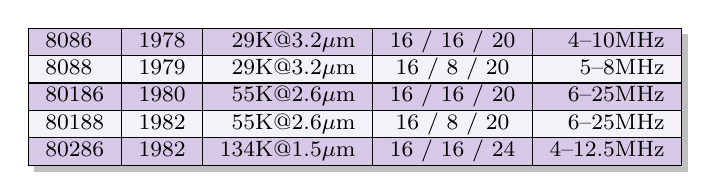
\begin{tikzpicture}
\node[drop shadow,fill=white,inner sep=0pt]
{\rowcolors{1}{RoyalPurple!20}{RoyalPurple!5}
{\footnotesize
\begin{tabular}{|l|r|r|c|r|}
\hline
8086 & 1978 & 29K@3.2$\mu$m & 16 / 16 / 20 & 4--10MHz \\
\hline
8088 & 1979 & 29K@3.2$\mu$m & 16 / 8 / 20 & 5--8MHz \\
\hline
80186 & 1980 & 55K@2.6$\mu$m & 16 / 16 / 20 & 6--25MHz \\
\hline
80188 & 1982 & 55K@2.6$\mu$m & 16 / 8 / 20 & 6--25MHz \\
\hline
80286 & 1982 & 134K@1.5$\mu$m & 16 / 16 / 24 & 4--12.5MHz \\
\hline
\end{tabular}%
}
};
\end{tikzpicture}
\end{center}
\end{frame}

\begin{frame}[t]{IA-32 CISC (Win 3.11, OS/2, Linux, BSD i386)}
\begin{block}{80386 (Am386, TI, Chips, IBM, \ldots)}
\begin{itemize}
\item IBM PS/2 (MCA). 32-bit segments, regs, buses
\item NatSemi 16550A UART. 80386SL: first (external) cache
\item 2\textbf{c} per simple instruction
\end{itemize}
\end{block}
\begin{block}{80486 (Am486, Cx486DLC, TI486SXL, IBM486DLC,\ldots)}
\begin{itemize}
\item EISA/VLB. On-die cache, \texttt{XADD}, \texttt{CMPXCHG}
\item 1\textbf{c} per simple instruction, integrated FPU
\end{itemize}
\end{block}
\vfill
\begin{center}
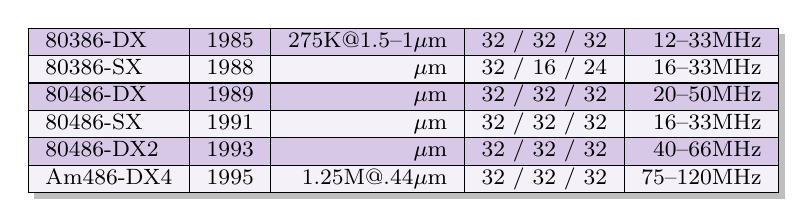
\begin{tikzpicture}
\node[drop shadow,fill=white,inner sep=0pt]
{\rowcolors{1}{RoyalPurple!20}{RoyalPurple!5}
{\footnotesize
\begin{tabular}{|l|r|r|c|r|}
\hline
80386-DX & 1985 & 275K@1.5--1$\mu$m & 32 / 32 / 32 & 12--33MHz \\
\hline
80386-SX & 1988 & $\mu$m & 32 / 16 / 24 & 16--33MHz \\
\hline
80486-DX & 1989 & $\mu$m & 32 / 32 / 32 & 20--50MHz \\
\hline
80486-SX & 1991 & $\mu$m & 32 / 32 / 32 & 16--33MHz \\
\hline
80486-DX2 & 1993 & $\mu$m & 32 / 32 / 32 & 40--66MHz \\
\hline
Am486-DX4 & 1995 & 1.25M@$.44\mu$m & 32 / 32 / 32 & 75--120MHz \\
\hline
\end{tabular}%
}
};
\end{tikzpicture}
\end{center}
\end{frame}

\begin{frame}[t]{MMX + superscalar (Win 95, BeOS, FreeBSD)}
\begin{block}{Intel Pentium}
\begin{itemize}
\item FIXME
\item PMMX adds MMX + performance counters (\texttt{RDPMC})
\end{itemize}
\end{block}
\begin{block}{AMD K5}
\begin{itemize}
\item FIXME
\end{itemize}
\end{block}
\vfill
\begin{center}
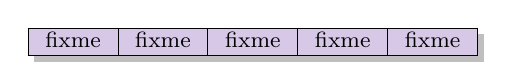
\begin{tikzpicture}
\node[drop shadow,fill=white,inner sep=0pt]
{\rowcolors{1}{RoyalPurple!20}{RoyalPurple!5}
{\footnotesize
\begin{tabular}{|l|r|r|c|r|}
\hline
fixme & fixme & fixme & fixme & fixme \\
\hline
\end{tabular}%
}
};
\end{tikzpicture}
\end{center}
\end{frame}

\begin{frame}[t]{SSE + OOO CRISC (Win 98, FreeBSD 3, Linux 2)}

\begin{block}{Intel P6 (PPro / PIII)}
\begin{itemize}
\item PPro adds \texttt{SYSENTER, SYSEXIT}
\item PIII adds 8 128-bit regs, SSE1 and \texttt{CMOVcc}
%SSE1 is strictly 32x4 FP + data-movement stuff, plus SFENCE
%PIII shared execution resources (save regs) between SSE/FP
\item FIXME
\end{itemize}
\end{block}
\begin{block}{AMD K6}
\begin{itemize}
\item Adds \texttt{SYSCALL, SYSRET}
\item K6-2 adds 3DNow! atop MMX regs
% shit for performance, but worked without OS support, but who cares?
\item FIXME
\end{itemize}
\end{block}
\vfill
\begin{center}
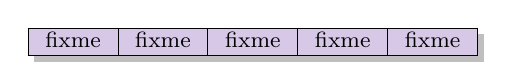
\begin{tikzpicture}
\node[drop shadow,fill=white,inner sep=0pt]
{\rowcolors{1}{RoyalPurple!20}{RoyalPurple!5}
{\footnotesize
\begin{tabular}{|l|r|r|c|r|}
\hline
fixme & fixme & fixme & fixme & fixme \\
\hline
\end{tabular}%
}
};
\end{tikzpicture}
\end{center}
\end{frame}

\begin{frame}[t]{SSE2 + long pipelines (FreeBSD 4, Linux 2.4)}
\begin{block}{Intel NetBurst (P4, PD)}
\begin{itemize}
\item P4 adds SSE2, HyperThreading
% SSE2 implements MMX integer ops and 64-bit double FP
\item FIXME
\end{itemize}
\end{block}
\begin{block}{AMD K7 (Athlon)}
\begin{itemize}
\item FIXME
\end{itemize}
\end{block}
\vfill
\begin{center}
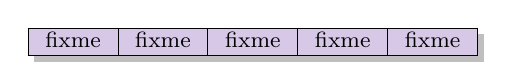
\begin{tikzpicture}
\node[drop shadow,fill=white,inner sep=0pt]
{\rowcolors{1}{RoyalPurple!20}{RoyalPurple!5}
{\footnotesize
\begin{tabular}{|l|r|r|c|r|}
\hline
fixme & fixme & fixme & fixme & fixme \\
\hline
\end{tabular}%
}
};
\end{tikzpicture}
\end{center}
\end{frame}

\begin{frame}[t]{IA-64 multicore (FreeBSD 7, Linux 2.6)}
\begin{block}{Intel Core}
\begin{itemize}
\item FIXME
\end{itemize}
\end{block}
\begin{block}{AMD K8}
\begin{itemize}
\item FIXME
\end{itemize}
\end{block}
\vfill
\begin{center}
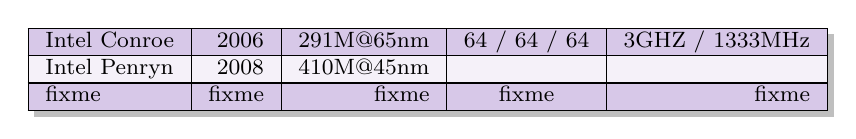
\begin{tikzpicture}
\node[drop shadow,fill=white,inner sep=0pt]
{\rowcolors{1}{RoyalPurple!20}{RoyalPurple!5}
{\footnotesize
\begin{tabular}{|l|r|r|c|r|}
\hline
Intel Conroe & 2006 & 291M@65nm & 64 / 64 / 64 & 3GHZ / 1333MHz \\
\hline
Intel Penryn & 2008 & 410M@45nm & & \\
\hline
fixme & fixme & fixme & fixme & fixme \\
\hline
\end{tabular}%
}
};
\end{tikzpicture}
\end{center}
\end{frame}

\begin{frame}[t]{AVX + scaling + heterogeneity (FreeBSD 8, Linux 3)}
\begin{block}{Intel Nehalem}
\begin{itemize}
\item Adds SSE4.2
\item Quick Path Interconnect on Nehalem-E
\item FIXME
\end{itemize}
\end{block}
\begin{block}{Intel Sandy Bridge / Ivy Bridge}
\begin{itemize}
\item PCIe 3.0 on Ivy Bridge
\item FIXME
\end{itemize}
\end{block}
\vfill
\begin{center}
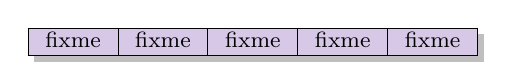
\begin{tikzpicture}
\node[drop shadow,fill=white,inner sep=0pt]
{\rowcolors{1}{RoyalPurple!20}{RoyalPurple!5}
{\footnotesize
\begin{tabular}{|l|r|r|c|r|}
\hline
fixme & fixme & fixme & fixme & fixme \\
\hline
\end{tabular}%
}
};
\end{tikzpicture}
\end{center}
\end{frame}

\end{document}
